\chapter{Evaluation}
The design of each strategy and the backtesting system allow for extensive parameterization, providing multiple axes for analysis. Parameters that can be adjusted are at what number of standard deviations away from the mean spread should a threshold set and a signal to be generated, how the trades are executed, limits on how much gas price should be when executing a trade, and also the volume of the initial investment. These are all factors that can effect the returns of the trading strategy. In the following sections, we will examine the performance of the strategy by varying these parameters, providing valuable insights into their influence on trading outcomes. For the purpose of data visualisation we denote the liquidity pool pairs by their index:
\begin{table}[!ht]
    \centering
    \begin{adjustwidth}{-0.5in}{-0.9in}
        \begin{tabular}{|p{20em}|p{20em}|p{3em}|}\hline
            Pool1 & Pool2 & Label\\\hline
            \truncate{20em}{USDC\_WETH\_0x88e6a0c2ddd26feeb64f039a2c41296fcb3f5640} & \truncate{20em}{USDC\_WETH\_0xe0554a476a092703abdb3ef35c80e0d76d32939f} & 0\\\hline
            \truncate{20em}{USDC\_WETH\_0x8ad599c3a0ff1de082011efddc58f1908eb6e6d8} & \truncate{20em}{USDC\_WETH\_0xe0554a476a092703abdb3ef35c80e0d76d32939f} & 1\\\hline
            \truncate{20em}{WETH\_USDT\_0x11b815efb8f581194ae79006d24e0d814b7697f6} & \truncate{20em}{USDC\_WETH\_0xe0554a476a092703abdb3ef35c80e0d76d32939f} & 2\\\hline
            \truncate{20em}{WETH\_USDT\_0x4e68ccd3e89f51c3074ca5072bbac773960dfa36} & \truncate{20em}{USDC\_WETH\_0xe0554a476a092703abdb3ef35c80e0d76d32939f} & 3\\\hline
            \truncate{20em}{DAI\_WETH\_0x60594a405d53811d3bc4766596efd80fd545a270} & \truncate{20em}{USDC\_WETH\_0xe0554a476a092703abdb3ef35c80e0d76d32939f} & 4\\\hline
            \truncate{20em}{DAI\_WETH\_0xc2e9f25be6257c210d7adf0d4cd6e3e881ba25f8} & \truncate{20em}{USDC\_WETH\_0xe0554a476a092703abdb3ef35c80e0d76d32939f} & 5\\\hline
            \truncate{20em}{USDC\_WETH\_0xe0554a476a092703abdb3ef35c80e0d76d32939f} & \truncate{20em}{WETH\_USDT\_0xc5af84701f98fa483ece78af83f11b6c38aca71d} & 6\\\hline
        \end{tabular}
    \end{adjustwidth}
    \caption{Liquidity pool pairs and their corresponding labels}
\end{table}
\vspace{-4ex}
\section{Number of Standard Deviations away from the Mean}
Varying the standard deviation in a mean reversion pairs trading strategy can have a significant impact on the strategy's returns. When the number of standard deviations is set too high, it means that the spread between the pair's prices must deviate significantly from the mean before a signal is generated. In this case, the strategy may generate fewer trades, resulting in longer holding periods for positions, however this tends to have a greater return per trade. On the other hand, setting a lower number of standard deviations makes the strategy more sensitive to smaller deviations from the mean. This increases the frequency of trade signals and potentially leads to more active trading. However, it also exposes the strategy to a higher risk of false signals or trading on noise in the price data. It can result in higher transaction costs and potentially lower returns due to increased trading activity, potentially resulting in losses. For the purpose of simplicity, $\#_{\sigma}$ denotes this parameter.
\\[5mm]
Table \ref{tab:varying_sigma} displays the returns as the standard deviations away from the mean the threshold is set. For the purpose of this experiment the other parameters were; 100 ETH worth of initial investment, the window size set to 30 days, a gas price threshold of 1 ETH (i.e. not having a threshold), the interactions with the blockchain to be seperately executed and finally the lag that the lagged strategy uses is set to 1 hour. The period that trading occurs is from 18th December 2021 to 9th June 2023.
\\[5mm]
We can see that as $\#_{\sigma} \rightarrow 0$, the number of trades increases however causes the returns to be more negative (and in some cases terminating early with 100\% loss) than positive, likely due to trades being opened when gas fees are substantially larger than the profit. However, if $\#_{\sigma}$ is larger, although the profits from each trade increases, the number of opportunities that were actionable were limited. Another interesting feature that can easily be spotted is that the Constant Hedge Ratio Strategy makes little to no profit in all cases whereas the other strategies perform better as $\#_{\sigma} \rightarrow \sim2$. Furthermore, all of the strategies return a profit on pool pair 6 with the exception of the Kalman Filter Strategy, albeit with a higher threshold.
\\[5mm]
Consistent profit among all of the pool pairs, excluding pool pair 6, is also achieved at different $\#_{\sigma}$s. We can see in Figure \ref{fig:varyStd} that the average return across all liquidity pool pairs that each strategy generates at each standard deviation. The Kalman Filter becomes largely profitable at $\#_{\sigma} = 0.5$, whereas the lagged, sliding window and granger causality strategies become profitable at $\#_{\sigma} = 2$. This is highly due to the fact that the Kalman Filter is better able to find underlying trends thus being better at selecting the hedge ratio.

\definecolor{green}{RGB}{0,153,0}
\begin{table}[!htb]
    \centering
    \begin{adjustwidth}{-0.8in}{-0.9in}
        \begin{tabular}{|p{4em}|p{2em}|p{3em}|p{3em}|p{3em}|p{3em}|p{3em}|p{3em}|p{3em}|p{3em}|p{3em}|p{3em}|}\hline
            Std & Pool Pair & \multicolumn{10}{|c|}{Strategy's Return - Trading from 18th December 2021 to 9th June 2023} \\\cline{3-12}
            &   & \multicolumn{2}{|c|}{Constant} & \multicolumn{2}{|c|}{Sliding Window} & \multicolumn{2}{|c|}{Lagged} & \multicolumn{2}{|c|}{Granger Causality} & \multicolumn{2}{|c|}{Kalman Filter}\\\cline{3-12}
            & & Return \% & \# of Trades & Return \% & \# of Trades & Return \% & \# of Trades & Return \% & \# of Trades & Return \% & \# of Trades\\\hline

            & 0 & \textcolor{green}{5.44} & 360 & \textcolor{green}{29.28} & 661 & \textcolor{green}{66.29} & 687 & \textcolor{green}{26.34} & 704 & \textcolor{green}{83.01} & 228\\\cline{3-12}
            & 1 & \textcolor{red}{-54.34} & 397 & \textcolor{red}{-83.7} & 660 & \textcolor{red}{-77.28} & 653 & \textcolor{red}{-85.49} & 680 & \textcolor{red}{-14.99} & 307\\\cline{3-12}
            & 2 & \textcolor{green}{5.83} & 454 & \textcolor{red}{-2.1} & 634 & \textcolor{green}{43.6} & 619 & \textcolor{red}{-4.04} & 730 & \textcolor{green}{89.13} & 236\\\cline{3-12}
            $\sigma=0.1$3 & \textcolor{red}{-67.51} & 535 & \textcolor{red}{-70.51} & 572 & \textcolor{red}{-73.24} & 604 & \textcolor{red}{-100} & 671 & \textcolor{red}{-14.05} & 301\\\cline{3-12}
            & 4 & \textcolor{green}{11.14} & 375 & \textcolor{green}{10.06} & 759 & \textcolor{green}{58.61} & 669 & \textcolor{green}{22.59} & 802 & \textcolor{green}{71.83} & 227\\\cline{3-12}
            & 5 & \textcolor{red}{-53.44} & 396 & \textcolor{red}{-75.16} & 587 & \textcolor{red}{-68.27} & 593 & \textcolor{red}{-100} & 587 & \textcolor{red}{-24.99} & 328\\\cline{3-12}
            & 6 & \textcolor{red}{-15.76} & 72 & \textcolor{red}{-82.0} & 213 & \textcolor{red}{-76.2} & 198 & \textcolor{red}{-75.63} & 195 & \textcolor{red}{-6.12} & 84\\\hline\hline

            & 0 & \textcolor{green}{11.77} & 723 & \textcolor{red}{-15.81} & 1223 & \textcolor{green}{104.48} & 1185 & \textcolor{red}{-2.31} & 1234 & \textcolor{green}{241.96} & 378\\\cline{3-12}
            & 1 & \textcolor{red}{-100} & 832 & \textcolor{red}{-100} & 920 & \textcolor{red}{-100} & 936 & \textcolor{red}{-100} & 978 & \textcolor{green}{60.2} & 456\\\cline{3-12}
            & 2 & \textcolor{green}{9.19} & 688 & \textcolor{red}{-0.88} & 1105 & \textcolor{green}{124.82} & 1025 & \textcolor{green}{35.78} & 1128 & \textcolor{green}{295.01} & 396\\\cline{3-12}
            $\sigma=0.5$& 3 & \textcolor{red}{-93.51} & 794 & \textcolor{red}{-100} & 944 & \textcolor{red}{-92.35} & 1063 & \textcolor{red}{-100} & 808 & \textcolor{green}{37.63} & 425\\\cline{3-12}
            & 4 & \textcolor{green}{26.01} & 826 & \textcolor{red}{-16.12} & 1243 & \textcolor{green}{112.45} & 1213 & \textcolor{green}{16.25} & 1217 & \textcolor{green}{244.51} & 391\\\cline{3-12}
            & 5 & \textcolor{red}{-95.02} & 837 & \textcolor{red}{-100} & 854 & \textcolor{red}{-100} & 905 & \textcolor{red}{-100} & 824 & \textcolor{green}{90.57} & 388\\\cline{3-12}
            & 6 & \textcolor{red}{-37.47} & 124 & \textcolor{red}{-96.69} & 359 & \textcolor{red}{-84.14} & 301 & \textcolor{red}{-95.26} & 367 & \textcolor{red}{-39.65} & 150\\\hline\hline
            
            & 0 & \textcolor{red}{-21.41} & 675 & \textcolor{red}{-1.59} & 864 & \textcolor{green}{129.7} & 865 & \textcolor{green}{20.4} & 913 & \textcolor{green}{164.34} & 442\\\cline{3-12}
            & 1 & \textcolor{red}{-100} & 791 & \textcolor{red}{-100} & 814 & \textcolor{red}{-93.81} & 1022 & \textcolor{red}{-100} & 818 & \textcolor{red}{-10.31} & 505\\\cline{3-12}
            & 2 & \textcolor{red}{-21.23} & 535 & \textcolor{green}{7.04} & 777 & \textcolor{green}{150.19} & 721 & \textcolor{green}{55.49} & 733 & \textcolor{green}{184.32} & 404\\\cline{3-12}
            $\sigma=1$ & 3 & \textcolor{red}{-100} & 497 & \textcolor{red}{-100} & 657 & \textcolor{red}{-74.92} & 872 & \textcolor{red}{-100} & 655 & \textcolor{green}{1.9} & 436\\\cline{3-12}
            & 4 & \textcolor{red}{-5.26} & 689 & \textcolor{green}{15.54} & 799 & \textcolor{green}{156.04} & 822 & \textcolor{green}{63.8} & 811 & \textcolor{green}{190.11} & 460\\\cline{3-12}
            & 5 & \textcolor{red}{-100} & 533 & \textcolor{red}{-100} & 612 & \textcolor{red}{-69.44} & 785 & \textcolor{red}{-85.49} & 766 & \textcolor{green}{37.38} & 408\\\cline{3-12}
            & 6 & \textcolor{red}{-53.08} & 108 & \textcolor{red}{-66.08} & 169 & \textcolor{red}{-46.79} & 125 & \textcolor{red}{-60.07} & 161 & \textcolor{red}{-41.59} & 158\\\hline\hline
            
            & 0 & \textcolor{green}{5.7} & 365 & \textcolor{green}{48.67} & 447 & \textcolor{green}{144.27} & 476 & \textcolor{green}{18.98} & 497 & \textcolor{green}{178.36} & 179\\\cline{3-12}
            & 1 & \textcolor{red}{-100} & 408 & \textcolor{red}{-63.97} & 509 & \textcolor{red}{-30.62} & 504 & \textcolor{red}{-66.71} & 507 & \textcolor{green}{68.75} & 221\\\cline{3-12}
            & 2 & \textcolor{red}{-6.09} & 302 & \textcolor{green}{22.37} & 402 & \textcolor{green}{115.76} & 391 & \textcolor{green}{25.89} & 371 & \textcolor{green}{171.74} & 147\\\cline{3-12}
            $\sigma=1.5$ & 3 & \textcolor{red}{-71.49} & 389 & \textcolor{red}{-58.55} & 453 & \textcolor{red}{-27.34} & 449 & \textcolor{red}{-63.59} & 436 & \textcolor{green}{79.79} & 166\\\cline{3-12}
            & 4 & \textcolor{red}{-12.11} & 324 & \textcolor{green}{38.58} & 428 & \textcolor{green}{128.86} & 426 & \textcolor{green}{18.33} & 431 & \textcolor{green}{176.14} & 201\\\cline{3-12}
            & 5 & \textcolor{red}{-100} & 312 & \textcolor{red}{-51.69} & 402 & \textcolor{red}{-2.83} & 379 & \textcolor{red}{-49.38} & 387 & \textcolor{green}{88.52} & 175\\\cline{3-12}
            & 6 & \textcolor{red}{-42.58} & 77 & \textcolor{red}{-40.18} & 87 & \textcolor{red}{-39.6} & 89 & \textcolor{red}{-32.75} & 83 & \textcolor{red}{-18.52} & 102\\\hline\hline
            
            & 0 & \textcolor{red}{-10.35} & 288 & \textcolor{green}{38.26} & 342 & \textcolor{green}{141.77} & 353 & \textcolor{green}{39.45} & 360 & \textcolor{green}{175.37} & 153\\\cline{3-12}
            & 1 & \textcolor{red}{-67.13} & 358 & \textcolor{red}{-29.23} & 293 & \textcolor{red}{-7.71} & 323 & \textcolor{red}{-32.4} & 305 & \textcolor{green}{74.13} & 178\\\cline{3-12}
            & 2 & \textcolor{red}{-2.51} & 225 & \textcolor{green}{33.15} & 277 & \textcolor{green}{115.65} & 270 & \textcolor{green}{29.04} & 258 & \textcolor{green}{167.95} & 133\\\cline{3-12}
            $\sigma=1.75$ & 3 & \textcolor{red}{-59.62} & 309 & \textcolor{red}{-21.28} & 268 & \textcolor{red}{-1.49} & 294 & \textcolor{red}{-22.82} & 260 & \textcolor{green}{88.24} & 145\\\cline{3-12}
            & 4 & \textcolor{red}{-3.72} & 241 & \textcolor{green}{41.37} & 294 & \textcolor{green}{92.24} & 291 & \textcolor{green}{38.18} & 302 & \textcolor{green}{146.99} & 152\\\cline{3-12}
            & 5 & \textcolor{red}{-54.88} & 287 & \textcolor{red}{-14.02} & 225 & \textcolor{green}{14.77} & 250 & \textcolor{red}{-11.38} & 228 & \textcolor{green}{103.61} & 152\\\cline{3-12}
            & 6 & \textcolor{red}{-47.31} & 76 & \textcolor{red}{-26.89} & 67 & \textcolor{red}{-40.81} & 76 & \textcolor{red}{-30.31} & 55 & \textcolor{red}{-22.66} & 74\\\hline\hline
            
            & 0 & \textcolor{green}{2.11} & 226 & \textcolor{green}{44.05} & 271 & \textcolor{green}{90.62} & 268 & \textcolor{green}{44.66} & 275 & \textcolor{green}{108.12} & 116\\\cline{3-12}
            & 1 & \textcolor{red}{-41.61} & 245 & \textcolor{green}{7.67} & 165 & \textcolor{green}{30.12} & 184 & \textcolor{green}{10.85} & 172 & \textcolor{green}{57.28} & 125\\\cline{3-12}
            & 2 & \textcolor{red}{-8.64} & 191 & \textcolor{green}{45.26} & 190 & \textcolor{green}{90.81} & 202 & \textcolor{green}{40.8} & 192 & \textcolor{green}{98.06} & 106\\\cline{3-12}
            $\sigma=2$ & 3 & \textcolor{red}{-48.82} & 228 & \textcolor{green}{5.81} & 160 & \textcolor{green}{24.92} & 178 & \textcolor{green}{5.27} & 155 & \textcolor{green}{57.92} & 121\\\cline{3-12}
            & 4 & \textcolor{green}{8.74} & 206 & \textcolor{green}{45.91} & 190 & \textcolor{green}{85.04} & 201 & \textcolor{green}{45.49} & 216 & \textcolor{green}{96.82} & 125\\\cline{3-12}
            & 5 & \textcolor{red}{-27.79} & 192 & \textcolor{green}{10.78} & 138 & \textcolor{green}{32.9} & 147 & \textcolor{green}{8.86} & 141 & \textcolor{green}{69.22} & 125\\\cline{3-12}
            & 6 & \textcolor{red}{-37.31} & 65 & \textcolor{red}{-22.0} & 49 & \textcolor{red}{-24.93} & 54 & \textcolor{red}{-19.7} & 45 & \textcolor{green}{0.99} & 53\\\hline\hline
            
            & 0 & \textcolor{green}{2.59} & 54 & \textcolor{green}{28.73} & 102 & \textcolor{green}{26.55} & 83 & \textcolor{green}{19.48} & 104 & \textcolor{green}{27.46} & 51\\\cline{3-12}
            & 1 & \textcolor{red}{-5.71} & 64 & \textcolor{green}{21.12} & 49 & \textcolor{green}{18.19} & 46 & \textcolor{green}{16.69} & 50 & \textcolor{green}{23.33} & 60\\\cline{3-12}
            & 2 & \textcolor{green}{1.95} & 61 & \textcolor{green}{20.39} & 56 & \textcolor{green}{22.55} & 64 & \textcolor{green}{14.05} & 62 & \textcolor{green}{21.34} & 52\\\cline{3-12}
            $\sigma=3$ & 3 & \textcolor{red}{-10.22} & 73 & \textcolor{green}{12.31} & 46 & \textcolor{green}{11.0} & 48 & \textcolor{green}{7.54} & 45 & \textcolor{green}{12.46} & 58\\\cline{3-12}
            & 4 & \textcolor{green}{4.65} & 67 & \textcolor{green}{32.37} & 57 & \textcolor{green}{28.98} & 64 & \textcolor{green}{29.66} & 61 & \textcolor{green}{26.45} & 57\\\cline{3-12}
            & 5 & \textcolor{red}{-6.49} & 53 & \textcolor{green}{20.89} & 39 & \textcolor{green}{18.45} & 39 & \textcolor{green}{13.41} & 42 & \textcolor{green}{26.67} & 57\\\cline{3-12}
            & 6 & \textcolor{red}{-1.72} & 13 & \textcolor{red}{-4.74} & 20 & \textcolor{red}{-3.19} & 25 & \textcolor{red}{-2.39} & 19 & \textcolor{green}{12.01} & 16\\\hline
        \end{tabular}
    \end{adjustwidth}
    \caption{Returns of various standard deviation thresholds of each strategy \label{tab:varying_sigma}}.
\end{table}

\begin{figure}[h!]
    \centering
    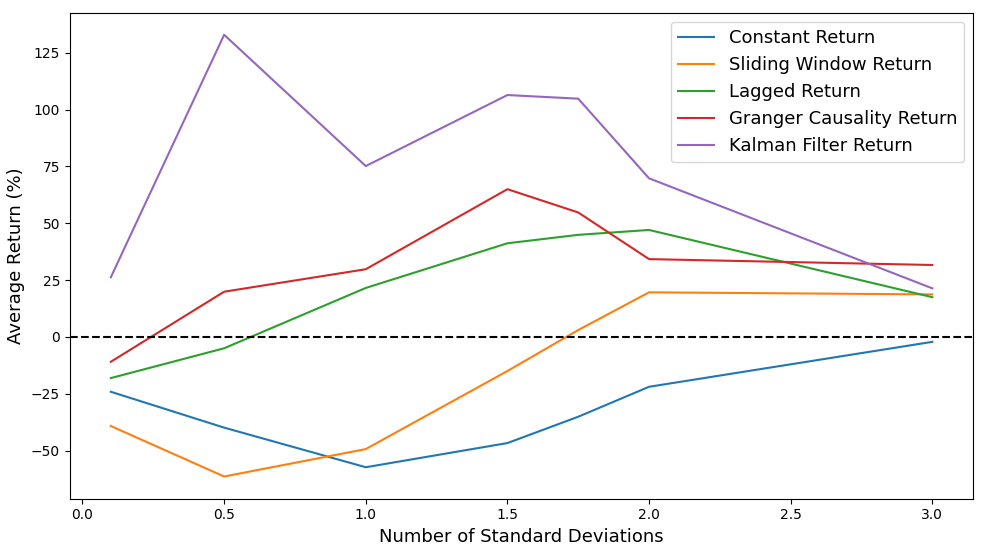
\includegraphics[width=1\textwidth]{evaluation/Images/VaryStd.png}
    \caption{Average Return across all pool pairs using various standard deviations}
    \label{fig:varyStd}
\end{figure}

\section{Gas Fees}
Another aspect that could be changed is fees; the first is how the transactions are executed on the blockchain and also the maximum gas price if we want to open a position. As previously mentioned, the gas fee is calculated by a combination of the gas price and the gas used. Therefore, these 2 parameters allow the strategy control both the gas used and gas price.

\subsection{Batched Transactions vs Seperately Executed Transactions}
The method in which the transactions are executed effects how much gas is used. When transactions are executed separately, each transaction incurs its own gas cost. This means that for every individual transaction, there will be gas consumed for various operations such as contract interaction, data storage, and computational tasks. As a result, executing a large number of separate transactions can lead to a significant cumulative gas cost. On the other hand, when transactions are batched together, they are consolidated into a single transaction. This consolidation reduces the overhead associated with executing multiple transactions individually. By combining the operations of multiple transactions into a single execution, redundant computations and storage operations can be eliminated, resulting in more efficient gas usage. It can immediately be seen in Figure  \ref{fig:gasResult} that the process of batching the transactions consumes less gas than the combined gas of the transactions required to exectue the openning and closing of the positions.
\\[5mm]
Furthermore, the effects of using seperate versus batched transactions can be seen in Table \ref{tab:BatchedVsSeperate}. The parameters used for this investigation were the same as above with the selection og $\sigma = 2$, 100 ETH worth of initial investment, the window size set to 30 days, a gas price threshold of 1 ETH (i.e. not having a threshold) and the testing period remained from 18th December 2021 to 9th June 2023.

\begin{table}[H]
    \centering
    \begin{adjustwidth}{-0.8in}{-0.9in}
        \begin{tabular}{|p{2em}|p{2em}|p{3em}|p{3em}|p{3em}|p{3em}|p{3em}|p{3em}|p{3em}|p{3em}|p{3em}|p{3em}|}\hline
            & Pool Pair & \multicolumn{10}{|c|}{Strategy's Return - Trading from 18th December 2021 to 9th June 2023} \\\cline{3-12}
            &   & \multicolumn{2}{|c|}{Constant} & \multicolumn{2}{|c|}{Sliding Window} & \multicolumn{2}{|c|}{Lagged} & \multicolumn{2}{|c|}{Granger Causality} & \multicolumn{2}{|c|}{Kalman Filter}\\\cline{3-12}
            & & Return \% & \# of Trades & Return \% & \# of Trades & Return \% & \# of Trades & Return \% & \# of Trades & Return \% & \# of Trades\\\hline
            
            \parbox[t]{4em}{\multirow{7}{*}{\rotatebox[origin=c]{90}{Seperate}}} & 0 & \textcolor{green}{2.11} & 226 & \textcolor{green}{44.05} & 271 & \textcolor{green}{90.62} & 268 & \textcolor{green}{44.66} & 275 & \textcolor{green}{108.12} & 116\\\cline{3-12}
            & 1 & \textcolor{red}{-41.61} & 245 & \textcolor{green}{7.67} & 165 & \textcolor{green}{30.12} & 184 & \textcolor{green}{10.85} & 172 & \textcolor{green}{57.28} & 125\\\cline{3-12}
            & 2 & \textcolor{red}{-8.64} & 191 & \textcolor{green}{45.26} & 190 & \textcolor{green}{90.81} & 202 & \textcolor{green}{40.8} & 192 & \textcolor{green}{98.06} & 106\\\cline{3-12}
            & 3 & \textcolor{red}{-48.82} & 228 & \textcolor{green}{5.81} & 160 & \textcolor{green}{24.92} & 178 & \textcolor{green}{5.27} & 155 & \textcolor{green}{57.92} & 121\\\cline{3-12}
            & 4 & \textcolor{green}{8.74} & 206 & \textcolor{green}{45.91} & 190 & \textcolor{green}{85.04} & 201 & \textcolor{green}{45.49} & 216 & \textcolor{green}{96.82} & 125\\\cline{3-12}
            & 5 & \textcolor{red}{-27.79} & 192 & \textcolor{green}{10.78} & 138 & \textcolor{green}{32.9} & 147 & \textcolor{green}{8.86} & 141 & \textcolor{green}{69.22} & 125\\\cline{3-12}
            & 6 & \textcolor{red}{-37.31} & 65 & \textcolor{red}{-22.0} & 49 & \textcolor{red}{-24.93} & 54 & \textcolor{red}{-19.7} & 45 & \textcolor{green}{0.99} & 53\\\hline\hline

            \parbox[t]{4em}{\multirow{7}{*}{\rotatebox[origin=c]{90}{Batched}}} & 0 & \textcolor{green}{6.81} & 226 & \textcolor{green}{50.16} & 271 & \textcolor{green}{98.85} & 268 & \textcolor{green}{49.96} & 275 & \textcolor{green}{110.51} & 116\\\cline{3-12}
            & 1 & \textcolor{red}{-38.34} & 245 & \textcolor{green}{10.25} & 165 & \textcolor{green}{34.9} & 184 & \textcolor{green}{13.73} & 172 & \textcolor{green}{59.82} & 125\\\cline{3-12}
            & 2 & \textcolor{red}{-3.11} & 191 & \textcolor{green}{49.14} & 190 & \textcolor{green}{94.82} & 202 & \textcolor{green}{46.1} & 192 & \textcolor{green}{101.01} & 106\\\cline{3-12}
            & 3 & \textcolor{red}{-44.85} & 228 & \textcolor{green}{8.45} & 160 & \textcolor{green}{28.38} & 178 & \textcolor{green}{8.56} & 155 & \textcolor{green}{60.58} & 121\\\cline{3-12}
            & 4 & \textcolor{green}{13.73} & 206 & \textcolor{green}{50.23} & 190 & \textcolor{green}{93.16} & 201 & \textcolor{green}{49.88} & 216 & \textcolor{green}{99.35} & 125\\\cline{3-12}
            & 5 & \textcolor{red}{-24.98} & 192 & \textcolor{green}{14.04} & 138 & \textcolor{green}{38.05} & 147 & \textcolor{green}{12.38} & 141 & \textcolor{green}{72.14} & 125\\\cline{3-12}
            & 6 & \textcolor{red}{-36.1} & 65 & \textcolor{red}{-20.65} & 49 & \textcolor{red}{-23.75} & 54 & \textcolor{red}{-18.66} & 45 & \textcolor{green}{1.93} & 53\\\hline
        \end{tabular}
    \end{adjustwidth}
    \caption{Returns of each strategy when using seperate and batched transactions \label{tab:BatchedVsSeperate}}.
\end{table}
\noindent When comparing the use of batched transactions to executing transactions separately, it is evident that utilizing batched transactions yields a higher return, as expected. The observed increase in return ranges from approximately 1\% to 8\% compared to executing the transactions individually. The higher return achieved through batched transactions can be attributed to several factors. First, as mentioned earlier, batching transactions reduces the gas costs associated with executing multiple transactions. By consolidating operations into a single transaction, redundant computations and storage operations are eliminated, resulting in more efficient gas usage. The reduction in gas costs directly contributes to the overall profitability of the trading strategy.

\subsection{Gas Price Threshold}
A threshold on the gas price is also set to ensure positions that have a high transaction cost associated with it are avoided. As the gas price is variable, we can see in Figure \ref{fig:GasPriceHistogram} the distribution of the gas prices over time is similar to a geometric distribution therefore by thresholding high gas prices, the strategies would avoid making a trade where the trade's profit would be overshadowed by the cost of trading.
\begin{figure}[h!]
    \centering
    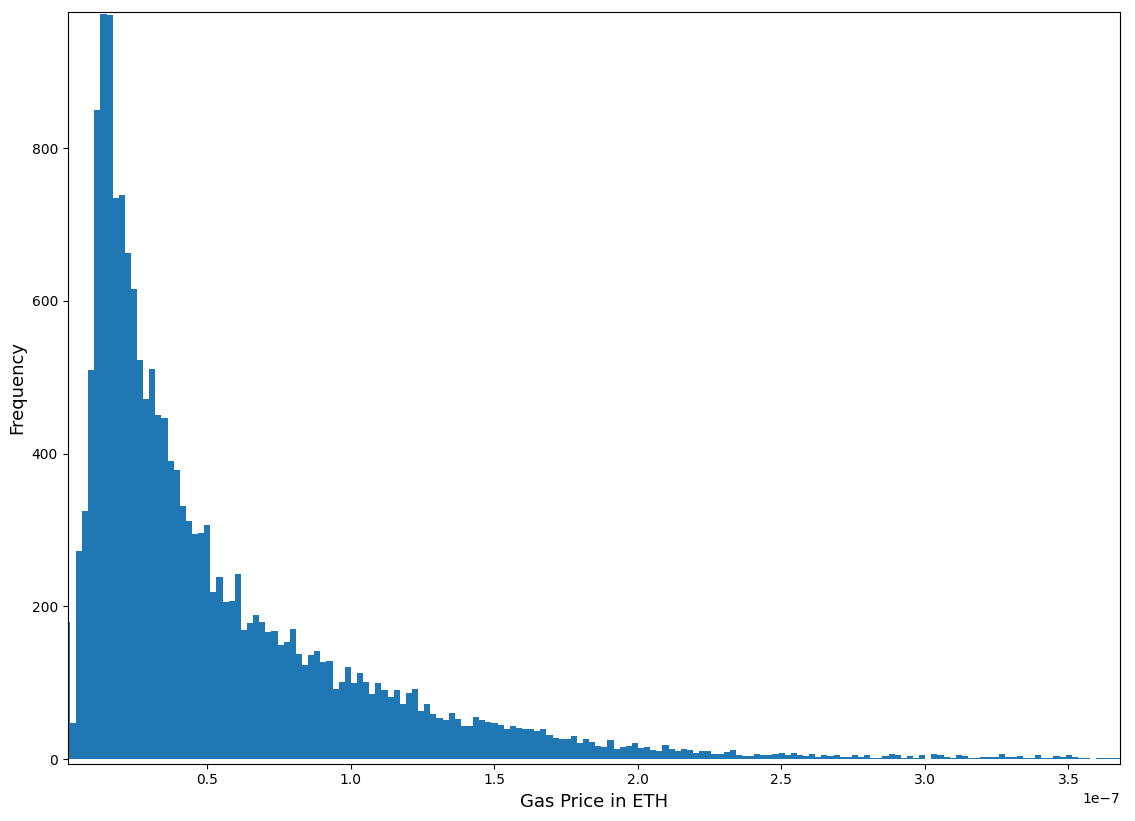
\includegraphics[width=\linewidth]{evaluation/Images/GasPriceHistogram.png}
    \caption{Histogram Plot of Gas Prices in ETH}
    \label{fig:GasPriceHistogram}
\end{figure}

\noindent Therefore, our investigation  consists of varying this threshold to see its effects on the returns of each strategy. Using batched transactions and the same parameters used in the aboce experiment, the thresholds are set to the $60^{th}, 70^{th},80^{th},90^{th},100^{th}$ quantiles. Table \ref{tab:VaryGasPriceThresholds} displays the results obtained by varying these thresholds. It can be seen that by filtering more costly opportunities, expectedly reduces the number of actionable, however the higher thresholds also show that these opportunities are still just as if not more profitable. In addition, to this Figure \ref{fig:VaryGasPriceThresholds}, shows that a low threshold benefits constant hedge ratio strategy most as with the low threshold, it has a light profit and as the threshold increases the return using the strategy decreases. Whereas, the returns are hindered with a lower threshold as many profitable opportunities are missed due to the overly low threshold, resulting in a reduction in the overall profitability of the trading strategy. The figure also shows how setting the threshold after the $90^{th}$ percentile does little to no effect in the return, giving a slight positive impact on the Lagged strategy and a slight negative impact on the the remaining. This is likely due to there only a small amounts of arbitrage opportunities to be present in such times when the gas price is high, thus having little impact. It is also interesting to see that the Lagged and the Kalman Filter strategies perform better by setting the threshold to the $90^{th}$ percentile in comparison to the $80^{th}$ percentile, whereas the other strategies perform worse.
\\[5mm]
Overall, the analysis of varying gas price thresholds reveals that adjusting the threshold level has a direct impact on the number of actionable opportunities and the resulting returns. Higher thresholds filter out less favorable opportunities, while still maintaining profitability. However, it is crucial to strike a balance and avoid setting the threshold too low, as this may lead to missed profitable opportunities. Hence, to get the best balance the threshold is set to the $90^{th}$ percentile.

\begin{figure}[H]
    \centering
    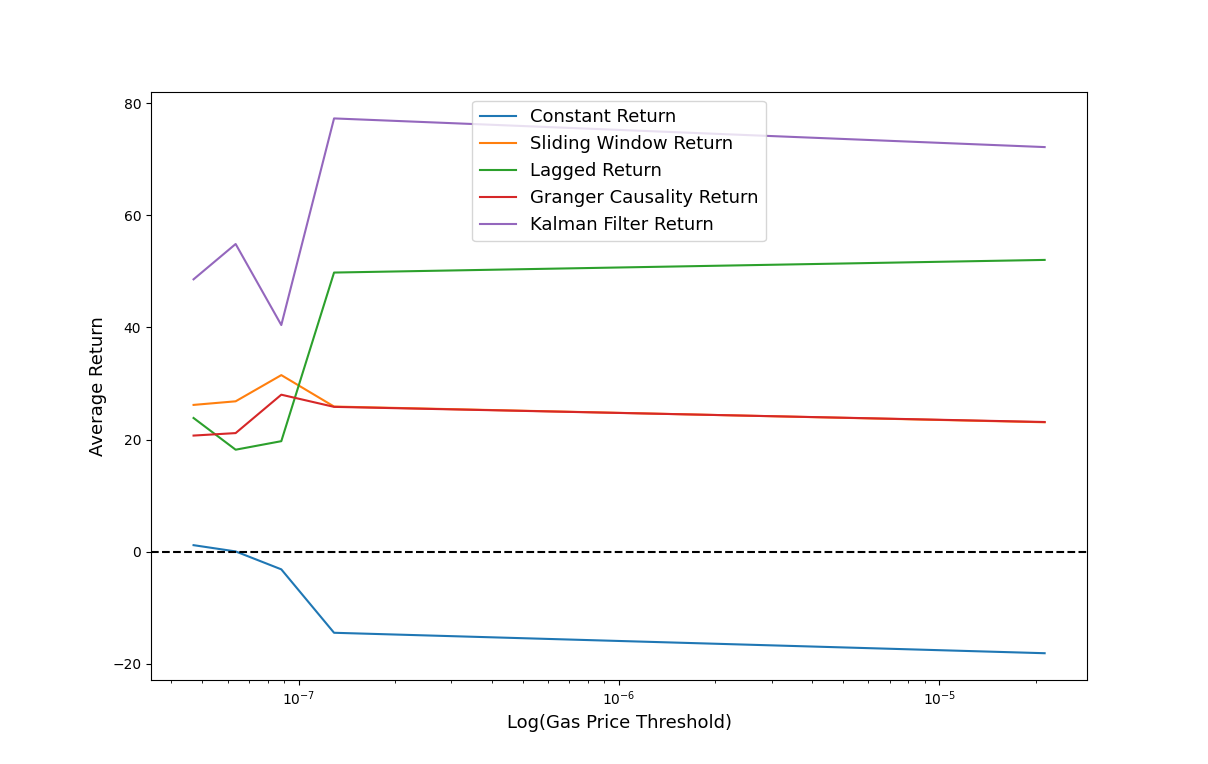
\includegraphics[width=\linewidth]{evaluation/Images/VaryGPThreshold.png}
    \caption{Average Returns of each strategy when using different gas price thresholds}
    \label{fig:VaryGasPriceThresholds}
\end{figure}

\begin{table}[htb!]
    \centering
    \begin{adjustwidth}{-0.9in}{-0.9in}
        \begin{tabular}{|p{5em}|p{2em}|p{3em}|p{3em}|p{3em}|p{3em}|p{3em}|p{3em}|p{3em}|p{3em}|p{3em}|p{3em}|}\hline
            Gas Price Threshold & Pool Pair & \multicolumn{10}{|c|}{Strategy's Return - Trading from 18th December 2021 to 9th June 2023} \\\cline{3-12}
            &   & \multicolumn{2}{|c|}{Constant} & \multicolumn{2}{|c|}{Sliding Window} & \multicolumn{2}{|c|}{Lagged} & \multicolumn{2}{|c|}{Granger Causality} & \multicolumn{2}{|c|}{Kalman Filter}\\\cline{3-12}
            & & Return \% & \# of Trades & Return \% & \# of Trades & Return \% & \# of Trades & Return \% & \# of Trades & Return \% & \# of Trades\\\hline
            
            & 0 & \textcolor{green}{22.72} & 150 & \textcolor{green}{34.17} & 176 & \textcolor{green}{39.52} & 177 & \textcolor{green}{30.81} & 182 & \textcolor{green}{64.96} & 74\\\cline{3-12}
            & 1 & \textcolor{red}{-11.82} & 172 & \textcolor{green}{24.13} & 81 & \textcolor{green}{22.54} & 94 & \textcolor{green}{19.46} & 87 & \textcolor{green}{41.1} & 79\\\cline{3-12}
            & 2 & \textcolor{green}{19.63} & 114 & \textcolor{green}{40.47} & 109 & \textcolor{green}{36.9} & 123 & \textcolor{green}{29.1} & 108 & \textcolor{green}{57.47} & 68\\\cline{3-12}
            $60^{th}$ percentile = 4.7e-08 & 3 & \textcolor{red}{-19.73} & 160 & \textcolor{green}{18.64} & 77 & \textcolor{green}{12.15} & 94 & \textcolor{green}{11.89} & 78 & \textcolor{green}{36.1} & 77\\[-5.5ex]\cline{3-12}
            & 4 & \textcolor{green}{25.65} & 137 & \textcolor{green}{47.56} & 103 & \textcolor{green}{46.48} & 110 & \textcolor{green}{43.35} & 122 & \textcolor{green}{67.37} & 83\\\cline{3-12}
            & 5 & \textcolor{red}{-0.96} & 131 & \textcolor{green}{28.1} & 66 & \textcolor{green}{24.97} & 69 & \textcolor{green}{21.4} & 70 & \textcolor{green}{58.88} & 83\\\cline{3-12}
            & 6 & \textcolor{red}{-27.37} & 41 & \textcolor{red}{-9.76} & 19 & \textcolor{red}{-15.59} & 30 & \textcolor{red}{-11.0} & 17 & \textcolor{green}{14.28} & 35\\\hline\hline

            & 0 & \textcolor{green}{25.0} & 175 & \textcolor{green}{42.21} & 203 & \textcolor{green}{36.98} & 203 & \textcolor{green}{35.46} & 209 & \textcolor{green}{80.35} & 86\\\cline{3-12}
            & 1 & \textcolor{red}{-13.87} & 190 & \textcolor{green}{23.04} & 105 & \textcolor{green}{12.27} & 122 & \textcolor{green}{18.52} & 113 & \textcolor{green}{46.1} & 96\\\cline{3-12}
            & 2 & \textcolor{green}{16.96} & 133 & \textcolor{green}{45.44} & 127 & \textcolor{green}{35.83} & 140 & \textcolor{green}{34.63} & 128 & \textcolor{green}{68.24} & 78\\\cline{3-12}
            $70^{th}$ percentile = 6.36e-08 & 3 & \textcolor{red}{-20.92} & 175 & \textcolor{green}{17.43} & 97 & \textcolor{green}{5.12} & 118 & \textcolor{green}{11.89} & 98 & \textcolor{green}{39.6} & 93\\[-5.5ex]\cline{3-12}
            & 4 & \textcolor{green}{24.58} & 158 & \textcolor{green}{43.3} & 125 & \textcolor{green}{39.47} & 132 & \textcolor{green}{38.82} & 147 & \textcolor{green}{80.53} & 95\\\cline{3-12}
            & 5 & \textcolor{red}{-6.39} & 149 & \textcolor{green}{27.68} & 81 & \textcolor{green}{16.46} & 88 & \textcolor{green}{21.4} & 86 & \textcolor{green}{64.56} & 94\\\cline{3-12}
            & 6 & \textcolor{red}{-25.06} & 48 & \textcolor{red}{-11.29} & 20 & \textcolor{red}{-18.77} & 38 & \textcolor{red}{-12.61} & 20 & \textcolor{green}{4.91} & 41\\\hline\hline
            
            & 0 & \textcolor{green}{23.24} & 191 & \textcolor{green}{50.8} & 220 & \textcolor{green}{42.52} & 222 & \textcolor{green}{51.77} & 227 & \textcolor{green}{62.22} & 93\\\cline{3-12}
            & 1 & \textcolor{red}{-16.23} & 206 & \textcolor{green}{22.35} & 122 & \textcolor{green}{8.58} & 140 & \textcolor{green}{24.11} & 130 & \textcolor{green}{30.6} & 103\\\cline{3-12}
            & 2 & \textcolor{green}{11.58} & 149 & \textcolor{green}{54.08} & 148 & \textcolor{green}{38.83} & 161 & \textcolor{green}{43.86} & 147 & \textcolor{green}{52.64} & 84\\\cline{3-12}
            $80^{th}$ percentile = 8.83e-08 & 3 & \textcolor{red}{-29.48} & 193 & \textcolor{green}{19.87} & 117 & \textcolor{green}{4.29} & 135 & \textcolor{green}{13.84} & 115 & \textcolor{green}{26.31} & 99\\[-5.5ex]\cline{3-12}
            & 4 & \textcolor{green}{22.55} & 176 & \textcolor{green}{56.57} & 146 & \textcolor{green}{43.9} & 153 & \textcolor{green}{52.29} & 170 & \textcolor{green}{64.64} & 102\\\cline{3-12}
            & 5 & \textcolor{red}{-5.81} & 162 & \textcolor{green}{31.25} & 100 & \textcolor{green}{17.66} & 108 & \textcolor{green}{25.47} & 104 & \textcolor{green}{47.57} & 100\\\cline{3-12}
            & 6 & \textcolor{red}{-27.93} & 51 & \textcolor{red}{-14.4} & 30 & \textcolor{red}{-17.77} & 41 & \textcolor{red}{-15.27} & 28 & \textcolor{red}{-0.92} & 42\\\hline\hline

            & 0 & \textcolor{green}{11.18} & 209 & \textcolor{green}{48.62} & 238 & \textcolor{green}{90.51} & 242 & \textcolor{green}{53.99} & 244 & \textcolor{green}{112.82} & 105\\\cline{3-12}
            & 1 & \textcolor{red}{-32.08} & 228 & \textcolor{green}{13.94} & 143 & \textcolor{green}{35.75} & 162 & \textcolor{green}{16.72} & 150 & \textcolor{green}{65.56} & 116\\\cline{3-12}
            & 2 & \textcolor{green}{2.72} & 171 & \textcolor{green}{49.32} & 164 & \textcolor{green}{81.65} & 181 & \textcolor{green}{46.37} & 165 & \textcolor{green}{99.58} & 96\\\cline{3-12}
            $90^{th}$ percentile = 1.29e-07 & 3 & \textcolor{red}{-40.06} & 212 & \textcolor{green}{13.44} & 137 & \textcolor{green}{28.08} & 158 & \textcolor{green}{12.52} & 133 & \textcolor{green}{60.31} & 111\\[-5.5ex]\cline{3-12}
            & 4 & \textcolor{green}{11.99} & 190 & \textcolor{green}{51.85} & 166 & \textcolor{green}{88.87} & 175 & \textcolor{green}{50.19} & 191 & \textcolor{green}{115.68} & 115\\\cline{3-12}
            & 5 & \textcolor{red}{-20.52} & 178 & \textcolor{green}{20.5} & 117 & \textcolor{green}{44.05} & 127 & \textcolor{green}{19.89} & 121 & \textcolor{green}{85.25} & 115\\\cline{3-12}
            & 6 & \textcolor{red}{-34.53} & 62 & \textcolor{red}{-16.41} & 39 & \textcolor{red}{-20.29} & 50 & \textcolor{red}{-18.82} & 39 & \textcolor{green}{1.94} & 47\\\hline\hline

            & 0 & \textcolor{green}{6.81} & 226 & \textcolor{green}{50.16} & 271 & \textcolor{green}{98.85} & 268 & \textcolor{green}{49.96} & 275 & \textcolor{green}{110.51} & 116\\\cline{3-12}
            & 1 & \textcolor{red}{-38.34} & 245 & \textcolor{green}{10.25} & 165 & \textcolor{green}{34.9} & 184 & \textcolor{green}{13.73} & 172 & \textcolor{green}{59.82} & 125\\\cline{3-12}
            & 2 & \textcolor{red}{-3.11} & 191 & \textcolor{green}{49.14} & 190 & \textcolor{green}{94.82} & 202 & \textcolor{green}{46.1} & 192 & \textcolor{green}{101.01} & 106\\\cline{3-12}
            $100^{th}$ percentile = 2.13e-05 & 3 & \textcolor{red}{-44.85} & 228 & \textcolor{green}{8.45} & 160 & \textcolor{green}{28.38} & 178 & \textcolor{green}{8.56} & 155 & \textcolor{green}{60.58} & 121\\[-5.5ex]\cline{3-12}
            & 4 & \textcolor{green}{13.73} & 206 & \textcolor{green}{50.23} & 190 & \textcolor{green}{93.16} & 201 & \textcolor{green}{49.88} & 216 & \textcolor{green}{99.35} & 125\\\cline{3-12}
            & 5 & \textcolor{red}{-24.98} & 192 & \textcolor{green}{14.04} & 138 & \textcolor{green}{38.05} & 147 & \textcolor{green}{12.38} & 141 & \textcolor{green}{72.14} & 125\\\cline{3-12}
            & 6 & \textcolor{red}{-36.1} & 65 & \textcolor{red}{-20.65} & 49 & \textcolor{red}{-23.75} & 54 & \textcolor{red}{-18.66} & 45 & \textcolor{green}{1.93} & 53\\\hline
        \end{tabular}
    \end{adjustwidth}
    \caption{Returns of each strategy when using different gas price thresholds \label{tab:VaryGasPriceThresholds}}.
\end{table}

\section{Initial Investment Volume}
Another import factor that contributes to the profit is the initial investment therefore Table \ref{tab:VaryInitialInvestments} and Figure \ref{fig:VaryInitialInvestments} displays the returns obtained by various initial investments. It can immediately be seen that the higher the investment, the greater the return. However, the smallest investments fall to a loss immediately for all strategies, this is because the fee that are incurred by gas fees are fixed regardless of the volume whereas the costs incurred by Aave and Uniswap are proportional to the volume being traded. This fixed fee means that a greater volume is required to cover the cost of the gas fee in order to generate profit, which is of course proportional to the volume being traded. Hence, as the investment increases the return increases however, begins to platau after 25ETH as the fixed fee becomes negligible in comparison to the investment.
\\[5mm]
Upon comparing the different strategies, the Kalman Filter is able to generate a profit with least amount of investment, followed by the Lagged strategy, then, interestingly, the Granger Causality and Sliding Window strategies perform exactly the same and finally the Constant strategy fails to make any money with any investment. This similarity between the Granger Causality and Sliding Window strategies is also evident in the other sections showing similar returns and trends as can be seen in Figures \ref{fig:varyStd} and \ref{fig:VaryGasPriceThresholds}.

\begin{figure}[H]
    \centering
    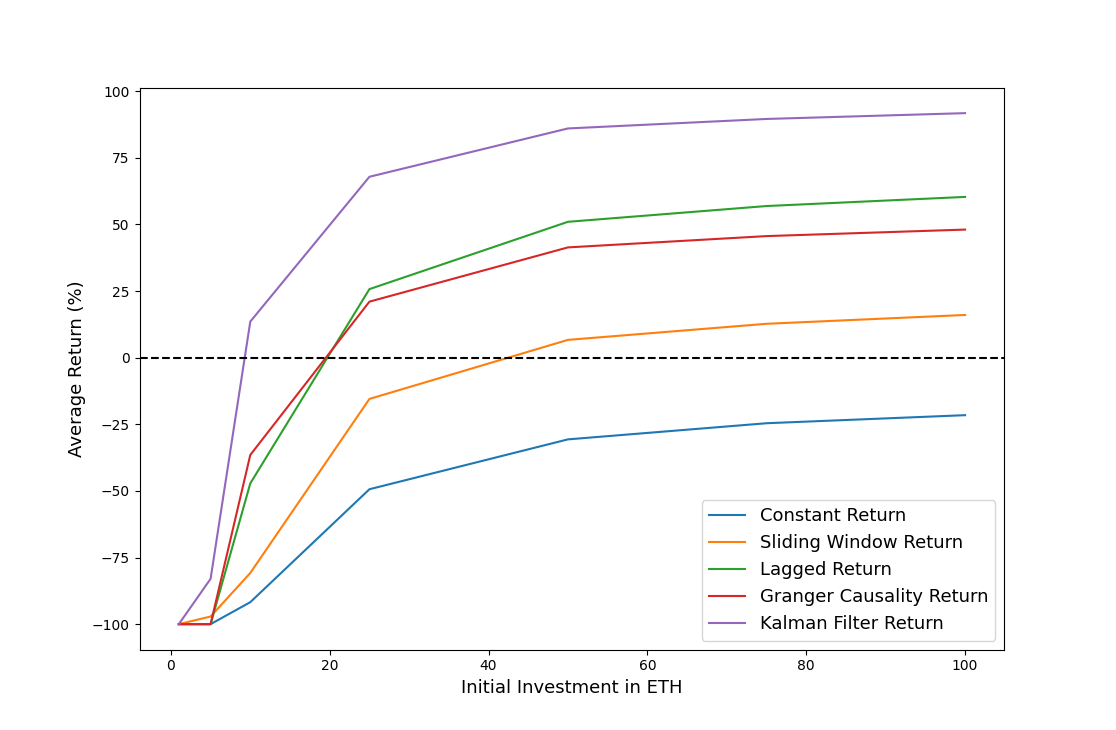
\includegraphics[width=\linewidth]{evaluation/Images/VaryII.png}
    \caption{Average Returns of each strategy using different initial investment volumes}
    \label{fig:VaryInitialInvestments}
\end{figure}

\begin{table}[htb!]
    \centering
    \begin{adjustwidth}{-0.9in}{-0.9in}
        \begin{tabular}{|p{5em}|p{2em}|p{3em}|p{3em}|p{3em}|p{3em}|p{3em}|p{3em}|p{3em}|p{3em}|p{3em}|p{3em}|}\hline
            Initial Investment & Pool Pair & \multicolumn{10}{|c|}{Strategy's Return - Trading from 18th December 2021 to 9th June 2023} \\\cline{3-12}
            &   & \multicolumn{2}{|c|}{Constant} & \multicolumn{2}{|c|}{Sliding Window} & \multicolumn{2}{|c|}{Lagged} & \multicolumn{2}{|c|}{Granger Causality} & \multicolumn{2}{|c|}{Kalman Filter}\\\cline{3-12}
            & & Return \% & \# of Trades & Return \% & \# of Trades & Return \% & \# of Trades & Return \% & \# of Trades & Return \% & \# of Trades\\\hline

            & 0 & \textcolor{red}{-100} & 4 & \textcolor{red}{-100} & 4 & \textcolor{red}{-100} & 3 & \textcolor{red}{-100} & 5 & \textcolor{red}{-100} & 2\\\cline{3-12}
            & 1 & \textcolor{red}{-100} & 4 & \textcolor{red}{-100} & 4 & \textcolor{red}{-100} & 3 & \textcolor{red}{-100} & 4 & \textcolor{red}{-100} & 2\\\cline{3-12}
            & 2 & \textcolor{red}{-100} & 4 & \textcolor{red}{-100} & 4 & \textcolor{red}{-100} & 3 & \textcolor{red}{-100} & 5 & \textcolor{red}{-100} & 2\\\cline{3-12}
            $1 ETH = \$3,946.26$ & 3 & \textcolor{red}{-100} & 4 & \textcolor{red}{-100} & 4 & \textcolor{red}{-100} & 3 & \textcolor{red}{-100} & 5 & \textcolor{red}{-100} & 2\\[-3ex]\cline{3-12}
            & 4 & \textcolor{red}{-100} & 4 & \textcolor{red}{-100} & 4 & \textcolor{red}{-100} & 3 & \textcolor{red}{-100} & 4 & \textcolor{red}{-100} & 3\\\cline{3-12}
            & 5 & \textcolor{red}{-100} & 4 & \textcolor{red}{-100} & 4 & \textcolor{red}{-100} & 3 & \textcolor{red}{-100} & 4 & \textcolor{red}{-100} & 3\\\cline{3-12}
            & 6 & \textcolor{red}{-100} & 3 & \textcolor{red}{-100} & 3 & \textcolor{red}{-100} & 2 & \textcolor{red}{-100} & 3 & \textcolor{red}{-100} & 1\\\hline\hline

            & 0 & \textcolor{red}{-100} & 101 & \textcolor{red}{-100} & 162 & \textcolor{red}{-100} & 183 & \textcolor{red}{-100} & 164 & \textcolor{red}{-27.63} & 105\\\cline{3-12}
            & 1 & \textcolor{red}{-100} & 58 & \textcolor{red}{-100} & 109 & \textcolor{red}{-100} & 129 & \textcolor{red}{-100} & 117 & \textcolor{red}{-64.03} & 116\\\cline{3-12}
            & 2 & \textcolor{red}{-100} & 93 & \textcolor{red}{-100} & 140 & \textcolor{red}{-100} & 157 & \textcolor{red}{-100} & 137 & \textcolor{red}{-26.65} & 96\\\cline{3-12}
            $5 ETH = \$19,731.30$ & 3 & \textcolor{red}{-100} & 83 & \textcolor{red}{-100} & 112 & \textcolor{red}{-100} & 130 & \textcolor{red}{-100} & 111 & \textcolor{red}{-60.74} & 111\\[-3ex]\cline{3-12}
            & 4 & \textcolor{red}{-100} & 86 & \textcolor{red}{-100} & 112 & \textcolor{red}{-100} & 152 & \textcolor{red}{-100} & 133 & \textcolor{red}{-34.43} & 115\\\cline{3-12}
            & 5 & \textcolor{red}{-100} & 77 & \textcolor{red}{-100} & 98 & \textcolor{red}{-100} & 108 & \textcolor{red}{-100} & 100 & \textcolor{red}{-52.21} & 115\\\cline{3-12}
            & 6 & \textcolor{red}{-85.23} & 62 & \textcolor{red}{-60.02} & 39 & \textcolor{red}{-67.01} & 50 & \textcolor{red}{-61.98} & 39 & \textcolor{red}{-49.09} & 47\\\hline\hline

            & 0 & \textcolor{red}{-80.81} & 209 & \textcolor{red}{-55.78} & 238 & \textcolor{red}{-25.22} & 242 & \textcolor{red}{-52.77} & 244 & \textcolor{green}{49.31} & 105\\\cline{3-12}
            & 1 & \textcolor{red}{-100} & 212 & \textcolor{red}{-56.48} & 143 & \textcolor{red}{-45.31} & 162 & \textcolor{red}{-54.56} & 150 & \textcolor{green}{6.44} & 116\\\cline{3-12}
            & 2 & \textcolor{red}{-74.22} & 171 & \textcolor{red}{-31.52} & 164 & \textcolor{red}{-11.64} & 181 & \textcolor{red}{-36.47} & 165 & \textcolor{green}{42.03} & 96\\\cline{3-12}
            $10 ETH = \$39,462.60$ & 3 & \textcolor{red}{-100} & 196 & \textcolor{red}{-50.92} & 137 & \textcolor{red}{-45.73} & 158 & \textcolor{red}{-48.65} & 133 & \textcolor{green}{5.61} & 111\\[-3ex]\cline{3-12}
            & 4 & \textcolor{red}{-72.54} & 190 & \textcolor{red}{-38.91} & 166 & \textcolor{red}{-11.69} & 175 & \textcolor{red}{-48.9} & 191 & \textcolor{green}{47.52} & 115\\\cline{3-12}
            & 5 & \textcolor{red}{-81.16} & 178 & \textcolor{red}{-40.14} & 117 & \textcolor{red}{-27.42} & 127 & \textcolor{red}{-40.67} & 121 & \textcolor{green}{22.3} & 115\\\cline{3-12}
            & 6 & \textcolor{red}{-58.01} & 62 & \textcolor{red}{-37.25} & 39 & \textcolor{red}{-42.5} & 50 & \textcolor{red}{-39.51} & 39 & \textcolor{red}{-21.73} & 47\\\hline\hline

            & 0 & \textcolor{red}{-19.01} & 209 & \textcolor{green}{14.13} & 238 & \textcolor{green}{51.64} & 242 & \textcolor{green}{18.52} & 244 & \textcolor{green}{94.82} & 105\\\cline{3-12}
            & 1 & \textcolor{red}{-56.47} & 228 & \textcolor{red}{-8.08} & 143 & \textcolor{green}{9.29} & 162 & \textcolor{red}{-5.72} & 150 & \textcolor{green}{45.24} & 116\\\cline{3-12}
            & 2 & \textcolor{red}{-22.95} & 171 & \textcolor{green}{22.08} & 164 & \textcolor{green}{52.42} & 181 & \textcolor{green}{18.66} & 165 & \textcolor{green}{80.01} & 96\\\cline{3-12}
            $25 ETH = \$98,656.50$ & 3 & \textcolor{red}{-61.21} & 212 & \textcolor{red}{-7.06} & 137 & \textcolor{green}{3.96} & 158 & \textcolor{red}{-7.51} & 133 & \textcolor{green}{41.42} & 111\\[-3ex]\cline{3-12}
            & 4 & \textcolor{red}{-14.86} & 190 & \textcolor{green}{21.34} & 166 & \textcolor{green}{55.75} & 175 & \textcolor{green}{19.35} & 191 & \textcolor{green}{95.92} & 115\\\cline{3-12}
            & 5 & \textcolor{red}{-40.57} & 178 & \textcolor{green}{1.78} & 117 & \textcolor{green}{23.11} & 127 & \textcolor{red}{-0.19} & 121 & \textcolor{green}{63.83} & 115\\\cline{3-12}
            & 6 & \textcolor{red}{-43.79} & 62 & \textcolor{red}{-23.67} & 39 & \textcolor{red}{-28.21} & 50 & \textcolor{red}{-26.08} & 39 & \textcolor{red}{-5.79} & 47\\\hline\hline

            & 0 & \textcolor{green}{1.29} & 209 & \textcolor{green}{38.06} & 238 & \textcolor{green}{79.34} & 242 & \textcolor{green}{43.18} & 244 & \textcolor{green}{107.37} & 105\\\cline{3-12}
            & 1 & \textcolor{red}{-39.83} & 228 & \textcolor{green}{6.6} & 143 & \textcolor{green}{27.67} & 162 & \textcolor{green}{9.23} & 150 & \textcolor{green}{59.83} & 116\\\cline{3-12}
            & 2 & \textcolor{red}{-5.27} & 171 & \textcolor{green}{41.2} & 164 & \textcolor{green}{73.06} & 181 & \textcolor{green}{38.2} & 165 & \textcolor{green}{94.67} & 96\\\cline{3-12}
            $50 ETH = \$197,313.00$ & 3 & \textcolor{red}{-46.81} & 212 & \textcolor{green}{6.87} & 137 & \textcolor{green}{21.85} & 158 & \textcolor{green}{5.92} & 133 & \textcolor{green}{55.0} & 111\\[-3ex]\cline{3-12}
            & 4 & \textcolor{green}{3.59} & 190 & \textcolor{green}{42.5} & 166 & \textcolor{green}{79.45} & 175 & \textcolor{green}{40.24} & 191 & \textcolor{green}{109.77} & 115\\\cline{3-12}
            & 5 & \textcolor{red}{-27.36} & 178 & \textcolor{green}{14.53} & 117 & \textcolor{green}{37.12} & 127 & \textcolor{green}{13.61} & 121 & \textcolor{green}{79.73} & 115\\\cline{3-12}
            & 6 & \textcolor{red}{-37.84} & 62 & \textcolor{red}{-18.83} & 39 & \textcolor{red}{-22.94} & 50 & \textcolor{red}{-21.24} & 39 & \textcolor{red}{-0.72} & 47\\\hline\hline

            & 0 & \textcolor{green}{8.16} & 209 & \textcolor{green}{45.11} & 238 & \textcolor{green}{86.54} & 242 & \textcolor{green}{50.2} & 244 & \textcolor{green}{111.08} & 105\\\cline{3-12}
            & 1 & \textcolor{red}{-34.67} & 228 & \textcolor{green}{11.44} & 143 & \textcolor{green}{32.94} & 162 & \textcolor{green}{14.26} & 150 & \textcolor{green}{63.6} & 116\\\cline{3-12}
            & 2 & \textcolor{green}{0.0} & 171 & \textcolor{green}{46.67} & 164 & \textcolor{green}{78.6} & 181 & \textcolor{green}{43.63} & 165 & \textcolor{green}{97.94} & 96\\\cline{3-12}
            $75 ETH = \$295,969.50$ & 3 & \textcolor{red}{-42.71} & 212 & \textcolor{green}{11.07} & 137 & \textcolor{green}{25.63} & 158 & \textcolor{green}{10.27} & 133 & \textcolor{green}{58.46} & 111\\[-3ex]\cline{3-12}
            & 4 & \textcolor{green}{9.19} & 190 & \textcolor{green}{48.86} & 166 & \textcolor{green}{85.49} & 175 & \textcolor{green}{46.94} & 191 & \textcolor{green}{113.77} & 115\\\cline{3-12}
            & 5 & \textcolor{red}{-22.95} & 178 & \textcolor{green}{18.4} & 117 & \textcolor{green}{41.63} & 127 & \textcolor{green}{17.75} & 121 & \textcolor{green}{83.38} & 115\\\cline{3-12}
            & 6 & \textcolor{red}{-35.63} & 62 & \textcolor{red}{-17.21} & 39 & \textcolor{red}{-21.17} & 50 & \textcolor{red}{-19.63} & 39 & \textcolor{green}{1.06} & 47\\\hline\hline

            & 0 & \textcolor{green}{11.18} & 209 & \textcolor{green}{48.62} & 238 & \textcolor{green}{90.51} & 242 & \textcolor{green}{53.99} & 244 & \textcolor{green}{112.82} & 105\\\cline{3-12}
            & 1 & \textcolor{red}{-32.08} & 228 & \textcolor{green}{13.94} & 143 & \textcolor{green}{35.75} & 162 & \textcolor{green}{16.72} & 150 & \textcolor{green}{65.56} & 116\\\cline{3-12}
            & 2 & \textcolor{green}{2.72} & 171 & \textcolor{green}{49.32} & 164 & \textcolor{green}{81.65} & 181 & \textcolor{green}{46.37} & 165 & \textcolor{green}{99.58} & 96\\\cline{3-12}
            $100 ETH = \$394,626.00$ & 3 & \textcolor{red}{-40.06} & 212 & \textcolor{green}{13.44} & 137 & \textcolor{green}{28.08} & 158 & \textcolor{green}{12.52} & 133 & \textcolor{green}{60.31} & 111\\[-3ex]\cline{3-12}
            & 4 & \textcolor{green}{11.99} & 190 & \textcolor{green}{51.85} & 166 & \textcolor{green}{88.87} & 175 & \textcolor{green}{50.19} & 191 & \textcolor{green}{115.68} & 115\\\cline{3-12}
            & 5 & \textcolor{red}{-20.52} & 178 & \textcolor{green}{20.5} & 117 & \textcolor{green}{44.05} & 127 & \textcolor{green}{19.89} & 121 & \textcolor{green}{85.25} & 115\\\cline{3-12}
            & 6 & \textcolor{red}{-34.53} & 62 & \textcolor{red}{-16.41} & 39 & \textcolor{red}{-20.29} & 50 & \textcolor{red}{-18.82} & 39 & \textcolor{green}{1.94} & 47\\\hline
        \end{tabular}
    \end{adjustwidth}
    \caption{Returns of each strategy when using different initial investment volumes (Note: Ethereum to USD conversion rate is from 18th December 2021) \label{tab:VaryInitialInvestments}}.
\end{table}

\section{Window Size}
The final parameter that also has an effect on the returns is the window size. This window size is used when calculating the mean and standard deviation that are used to calculate the thresholds. As we can see in the excerpt below, the greater the window size, the more data the strategy would use to calculate the thresholds.
\vspace{5mm}
\begin{lstlisting}[language=Python]
spread = self.history_p1[-self.window_size_in_hours:] - self.hedge_ratio * self.history_p2[-self.window_size_in_hours:]
spread_mean = spread.mean()
spread_std = spread.std()
self.upper_threshold = spread_mean + self.number_of_sds_from_mean * spread_std
self.lower_threshold = spread_mean - self.number_of_sds_from_mean * spread_std
\end{lstlisting}
\vspace{5mm}
To evaluate how the window size effects the returns, backtesting is conducted over the period 9th June 2022 to the 9th June 2023, exactly 1 year. The results can be found in Table \ref{tab:VaryWS} and Figure \ref{fig:VaryWS} where we can see that, as the window sizes increase, the returns increase however for the smaller window sizes, the return are more eratic and volatile. This volatility decreases as the window size is increases platauing to each strategies respective returns.
\\[5mm]
It is also interesting to see that in this period of trading the Kalman Filter performs the worst which is surprising as in has outperformed each of the strategies in the experiment that have been previously mentioned.

\begin{figure}[H]
    \centering
    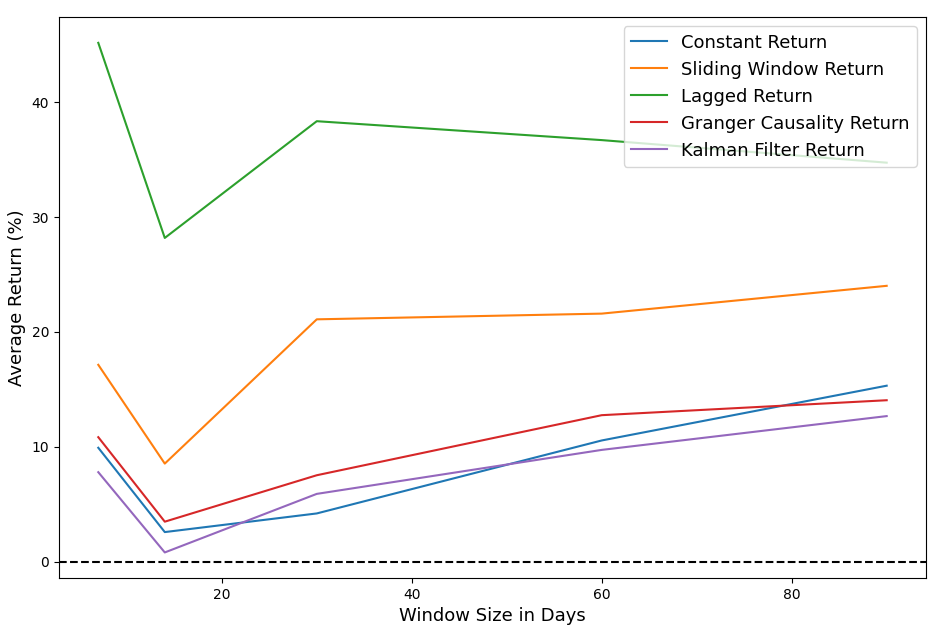
\includegraphics[width=\linewidth]{evaluation/Images/VarWS.png}
    \caption{Average Returns of each strategy using different Window Sizes}
    \label{fig:VaryWS}
\end{figure}

\begin{table}[!htb]
    \centering
    \begin{adjustwidth}{-0.8in}{-0.9in}
        \begin{tabular}{|p{4em}|p{2em}|p{3em}|p{3em}|p{3em}|p{3em}|p{3em}|p{3em}|p{3em}|p{3em}|p{3em}|p{3em}|}\hline
            Window Size & Pool Pair & \multicolumn{10}{|c|}{Strategy's Return - Trading from 9th June 2022 to the 9th June 2023} \\\cline{3-12}
            &   & \multicolumn{2}{|c|}{Constant} & \multicolumn{2}{|c|}{Sliding Window} & \multicolumn{2}{|c|}{Lagged} & \multicolumn{2}{|c|}{Granger Causality} & \multicolumn{2}{|c|}{Kalman Filter}\\\cline{3-12}
            & & Return \% & \# of Trades & Return \% & \# of Trades & Return \% & \# of Trades & Return \% & \# of Trades & Return \% & \# of Trades\\\hline

            & 0 & \textcolor{green}{29.57} & 287 & \textcolor{green}{42.3} & 230 & \textcolor{green}{73.88} & 233 & \textcolor{green}{30.42} & 252 & \textcolor{green}{23.53} & 271\\\cline{3-12}
            & 1 & \textcolor{red}{-0.77} & 182 & \textcolor{green}{5.81} & 150 & \textcolor{green}{26.1} & 175 & \textcolor{green}{1.27} & 144 & \textcolor{green}{1.48} & 142\\\cline{3-12}
            & 2 & \textcolor{green}{33.63} & 252 & \textcolor{green}{31.28} & 220 & \textcolor{green}{66.32} & 205 & \textcolor{green}{27.2} & 214 & \textcolor{green}{22.12} & 211\\\cline{3-12}
            7 days & 3 & \textcolor{red}{-8.07} & 185 & \textcolor{green}{1.44} & 151 & \textcolor{green}{22.42} & 168 & \textcolor{red}{-3.93} & 146 & \textcolor{red}{-0.98} & 141\\\cline{3-12}
            & 4 & \textcolor{green}{25.2} & 249 & \textcolor{green}{35.35} & 225 & \textcolor{green}{72.91} & 226 & \textcolor{green}{23.7} & 231 & \textcolor{green}{32.57} & 249\\\cline{3-12}
            & 5 & \textcolor{green}{5.04} & 132 & \textcolor{green}{9.19} & 113 & \textcolor{green}{41.86} & 132 & \textcolor{green}{7.02} & 103 & \textcolor{green}{4.98} & 108\\\cline{3-12}
            & 6 & \textcolor{red}{-15.21} & 42 & \textcolor{red}{-5.42} & 40 & \textcolor{green}{12.7} & 35 & \textcolor{red}{-9.84} & 34 & \textcolor{red}{-29.19} & 62\\\hline\hline

            & 0 & \textcolor{green}{15.64} & 249 & \textcolor{green}{18.97} & 221 & \textcolor{green}{53.47} & 233 & \textcolor{green}{15.29} & 254 & \textcolor{green}{16.32} & 220\\\cline{3-12}
            & 1 & \textcolor{red}{-2.75} & 161 & \textcolor{green}{1.28} & 127 & \textcolor{green}{15.18} & 154 & \textcolor{red}{-4.86} & 136 & \textcolor{red}{-6.22} & 124\\\cline{3-12}
            & 2 & \textcolor{green}{12.32} & 223 & \textcolor{green}{20.42} & 204 & \textcolor{green}{44.04} & 228 & \textcolor{green}{14.21} & 201 & \textcolor{green}{9.71} & 203\\\cline{3-12}
            14 days & 3 & \textcolor{red}{-15.12} & 176 & \textcolor{red}{-6.42} & 132 & \textcolor{green}{6.98} & 161 & \textcolor{red}{-13.09} & 131 & \textcolor{red}{-17.25} & 159\\\cline{3-12}
            & 4 & \textcolor{green}{20.55} & 220 & \textcolor{green}{22.92} & 188 & \textcolor{green}{46.76} & 197 & \textcolor{green}{16.48} & 208 & \textcolor{green}{18.3} & 182\\\cline{3-12}
            & 5 & \textcolor{green}{0.95} & 123 & \textcolor{green}{8.35} & 95 & \textcolor{green}{21.37} & 125 & \textcolor{green}{2.81} & 102 & \textcolor{red}{-1.34} & 105\\\cline{3-12}
            & 6 & \textcolor{red}{-13.59} & 29 & \textcolor{red}{-5.78} & 31 & \textcolor{green}{9.48} & 20 & \textcolor{red}{-6.5} & 31 & \textcolor{red}{-13.93} & 32\\\hline\hline
            
            & 0 & \textcolor{green}{21.12} & 207 & \textcolor{green}{32.86} & 205 & \textcolor{green}{61.17} & 197 & \textcolor{green}{18.65} & 237 & \textcolor{green}{29.15} & 254\\\cline{3-12}
            & 1 & \textcolor{red}{-15.8} & 198 & \textcolor{green}{12.41} & 111 & \textcolor{green}{27.29} & 117 & \textcolor{red}{-1.61} & 135 & \textcolor{red}{-8.44} & 153\\\cline{3-12}
            & 2 & \textcolor{green}{22.24} & 155 & \textcolor{green}{35.21} & 136 & \textcolor{green}{55.67} & 142 & \textcolor{green}{16.04} & 148 & \textcolor{green}{17.91} & 170\\\cline{3-12}
            30 days & 3 & \textcolor{red}{-15.71} & 178 & \textcolor{green}{9.32} & 101 & \textcolor{green}{22.54} & 114 & \textcolor{red}{-4.67} & 113 & \textcolor{red}{-12.4} & 155\\\cline{3-12}
            & 4 & \textcolor{green}{21.07} & 180 & \textcolor{green}{41.27} & 137 & \textcolor{green}{58.07} & 132 & \textcolor{green}{26.92} & 172 & \textcolor{green}{26.21} & 186\\\cline{3-12}
            & 5 & \textcolor{green}{0.13} & 140 & \textcolor{green}{17.82} & 81 & \textcolor{green}{36.66} & 81 & \textcolor{green}{7.29} & 92 & \textcolor{red}{-2.01} & 129\\\cline{3-12}
            & 6 & \textcolor{red}{-3.69} & 21 & \textcolor{red}{-1.22} & 24 & \textcolor{green}{7.03} & 15 & \textcolor{red}{-9.98} & 21 & \textcolor{red}{-9.14} & 20\\\hline\hline

            & 0 & \textcolor{green}{23.26} & 232 & \textcolor{green}{39.1} & 234 & \textcolor{green}{53.18} & 233 & \textcolor{green}{33.79} & 237 & \textcolor{green}{21.36} & 233\\\cline{3-12}
            & 1 & \textcolor{red}{-1.49} & 118 & \textcolor{green}{6.38} & 112 & \textcolor{green}{24.68} & 106 & \textcolor{green}{0.67} & 128 & \textcolor{red}{-1.68} & 112\\\cline{3-12}
            & 2 & \textcolor{green}{19.33} & 88 & \textcolor{green}{27.29} & 79 & \textcolor{green}{49.65} & 72 & \textcolor{green}{19.62} & 83 & \textcolor{green}{17.2} & 75\\\cline{3-12}
            60 days & 3 & \textcolor{green}{2.29} & 80 & \textcolor{green}{9.32} & 61 & \textcolor{green}{35.81} & 53 & \textcolor{green}{5.01} & 65 & \textcolor{red}{-2.89} & 75\\\cline{3-12}
            & 4 & \textcolor{green}{25.53} & 105 & \textcolor{green}{40.58} & 97 & \textcolor{green}{57.12} & 93 & \textcolor{green}{25.4} & 115 & \textcolor{green}{25.95} & 98\\\cline{3-12}
            & 5 & \textcolor{green}{12.35} & 53 & \textcolor{green}{32.81} & 44 & \textcolor{green}{41.18} & 47 & \textcolor{green}{15.33} & 54 & \textcolor{green}{14.45} & 48\\\cline{3-12}
            & 6 & \textcolor{red}{-7.43} & 24 & \textcolor{red}{-4.33} & 24 & \textcolor{red}{-4.71} & 24 & \textcolor{red}{-10.57} & 26 & \textcolor{red}{-6.3} & 25\\\hline\hline

            & 0 & \textcolor{green}{26.57} & 269 & \textcolor{green}{45.71} & 272 & \textcolor{green}{51.48} & 266 & \textcolor{green}{29.2} & 265 & \textcolor{green}{27.05} & 271\\\cline{3-12}
            & 1 & \textcolor{green}{3.09} & 111 & \textcolor{green}{9.17} & 109 & \textcolor{green}{19.79} & 114 & \textcolor{green}{2.62} & 116 & \textcolor{green}{0.42} & 110\\\cline{3-12}
            & 2 & \textcolor{green}{24.38} & 54 & \textcolor{green}{31.02} & 51 & \textcolor{green}{40.09} & 51 & \textcolor{green}{22.79} & 52 & \textcolor{green}{20.87} & 49\\\cline{3-12}
            90 days & 3 & \textcolor{green}{10.46} & 57 & \textcolor{green}{19.31} & 49 & \textcolor{green}{28.97} & 46 & \textcolor{green}{8.07} & 47 & \textcolor{green}{5.11} & 47\\\cline{3-12}
            & 4 & \textcolor{green}{32.58} & 85 & \textcolor{green}{46.23} & 83 & \textcolor{green}{57.24} & 78 & \textcolor{green}{28.66} & 86 & \textcolor{green}{30.72} & 87\\\cline{3-12}
            & 5 & \textcolor{green}{16.96} & 51 & \textcolor{green}{24.71} & 50 & \textcolor{green}{49.7} & 47 & \textcolor{green}{16.17} & 55 & \textcolor{green}{12.96} & 52\\\cline{3-12}
            & 6 & \textcolor{red}{-6.82} & 24 & \textcolor{red}{-8.06} & 26 & \textcolor{red}{-4.12} & 24 & \textcolor{red}{-9.15} & 25 & \textcolor{red}{-8.44} & 25\\\hline
            
        \end{tabular}
    \end{adjustwidth}
    \caption{Returns of various standard deviation thresholds of each strategy \label{tab:VaryWS}}.
\end{table}

\section{Evaluation of Strategies}
Overall, given the experiments conducted the optimal paramters for each strategy are different and thus to evaluate each strategy, the following paramters are used:

\begin{table}[H]
    \centering
    \begin{tabular}{|p{4em}|p{8em}|p{4em}|p{4em}|p{4em}|p{8em}|}
    \hline
        Strategy & Number of Standard Deviations from the mean, $\#_{\sigma}$ & Gas Price Threshold in ETH & Initial Investment in ETH & Window Size in Days & Type of Execution, Seperate or Batched \\ \hline
        Constant & 3 & 4.7E-08 & 100 & 60 & Batched \\ \hline
        Sliding Window & 2 & 8.83E-08 & 100 & 60 & Batched \\ \hline
        Lagged & 2 & 1.29E-07 & 100 & 30 & Batched \\ \hline
        Granger Causality & 2 & 8.83E-08 & 100 & 60 & Batched \\ \hline
        Kalman Filter & 0.5 & 1.29E-07 & 100 & 30 & Batched \\ \hline
    \end{tabular}
    \caption{Optimal Parameters for each strategy \label{tab:OptimParams}}
\end{table}

By running the backtesting system from 18th December 2021 to 9th June 2023, we can see in Table \ref{tab:FinalResults} the Kalman Filter outperforms all of the other strategies in all liquidity pool pairs except pair 6. The Lagged strategy has also performed well, whereas the Constant, Granger Causality and the Sliding Window strategies also resulting in similar mediocre returns, with the Granger Causality strategy performing the worst.

\begin{table}[!htb]
    \centering
    \begin{adjustwidth}{-0.8in}{-0.9in}
        \begin{tabular}{|p{4em}|p{3em}|p{3em}|p{3em}|p{3em}|p{3em}|p{3em}|p{3em}|p{3em}|p{3em}|p{3em}|}\hline
            Pool Pair & \multicolumn{10}{|c|}{Strategy's APR - Trading from 18th December 2021 to 9th June 2023} \\\cline{2-11}
            & \multicolumn{2}{|c|}{Constant} & \multicolumn{2}{|c|}{Sliding Window} & \multicolumn{2}{|c|}{Lagged} & \multicolumn{2}{|c|}{Granger Causality} & \multicolumn{2}{|c|}{Kalman Filter}\\\cline{2-11}
            & Return \% & \# of Trades & Return \% & \# of Trades & Return \% & \# of Trades & Return \% & \# of Trades & Return \% & \# of Trades\\\hline
            0 & \textcolor{green}{33.47} & 75 & \textcolor{green}{57.95} & 250 & \textcolor{green}{90.51} & 242 & \textcolor{green}{55.36} & 250 & \textcolor{green}{267.18} & 354\\\cline{2-11}
            1 & \textcolor{green}{32.46} & 32 & \textcolor{green}{20.7} & 127 & \textcolor{green}{35.75} & 162 & \textcolor{green}{8.83} & 136 & \textcolor{green}{82.26} & 425\\\cline{2-11}
            2 & \textcolor{green}{30.48} & 44 & \textcolor{green}{45.55} & 103 & \textcolor{green}{81.65} & 181 & \textcolor{green}{38.55} & 104 & \textcolor{green}{297.14} & 371\\\cline{2-11}
            3 & \textcolor{green}{24.94} & 29 & \textcolor{green}{20.52} & 86 & \textcolor{green}{28.08} & 158 & \textcolor{green}{11.02} & 94 & \textcolor{green}{48.13} & 399\\\cline{2-11}
            4 & \textcolor{green}{38.87} & 42 & \textcolor{green}{57.69} & 122 & \textcolor{green}{88.87} & 175 & \textcolor{green}{40.3} & 139 & \textcolor{green}{270.08} & 363\\\cline{2-11}
            5 & \textcolor{green}{31.17} & 24 & \textcolor{green}{37.84} & 77 & \textcolor{green}{44.05} & 127 & \textcolor{green}{23.78} & 83 & \textcolor{green}{96.64} & 366\\\cline{2-11}
            6 & \textcolor{red}{-2.46} & 13 & \textcolor{red}{-14.07} & 30 & \textcolor{red}{-20.29} & 50 & \textcolor{red}{-16.96} & 27 & \textcolor{red}{-31.93} & 147\\\hline\hline           
            Average & \textcolor{green}{26.99} & 37 & \textcolor{green}{32.31} & 113.6 & \textcolor{green}{49.80} & 156.4 & \textcolor{green}{22.98} & 119 & \textcolor{green}{147.07} & 346.4\\\hline            
            Average of APR return of each pool pair & \textcolor{green}{18.48} &  & \textcolor{green}{21.70} &   & \textcolor{green}{32.52} &  & \textcolor{green}{15.51} &  & \textcolor{green}{85.64} & \\\hline            
        \end{tabular}
    \end{adjustwidth}
    \caption{Returns of each strategy with their optimal parameters \label{tab:FinalResults}}.
\end{table}

In addition to this, Figure \ref{fig:ValueHistory} shows the account value over time of each of the strategies, it is easy the see that the account values seem to follow a trend however, the gradients of the return are less drastic in some strategies i.e. the Kalman Filter. It is also notable that the number of profitable trades and decreased since the beginning of 2023, with the Kalman Filter strategy taking a large loss in January of this year, 2023.

\begin{figure}[H]
    \centering
    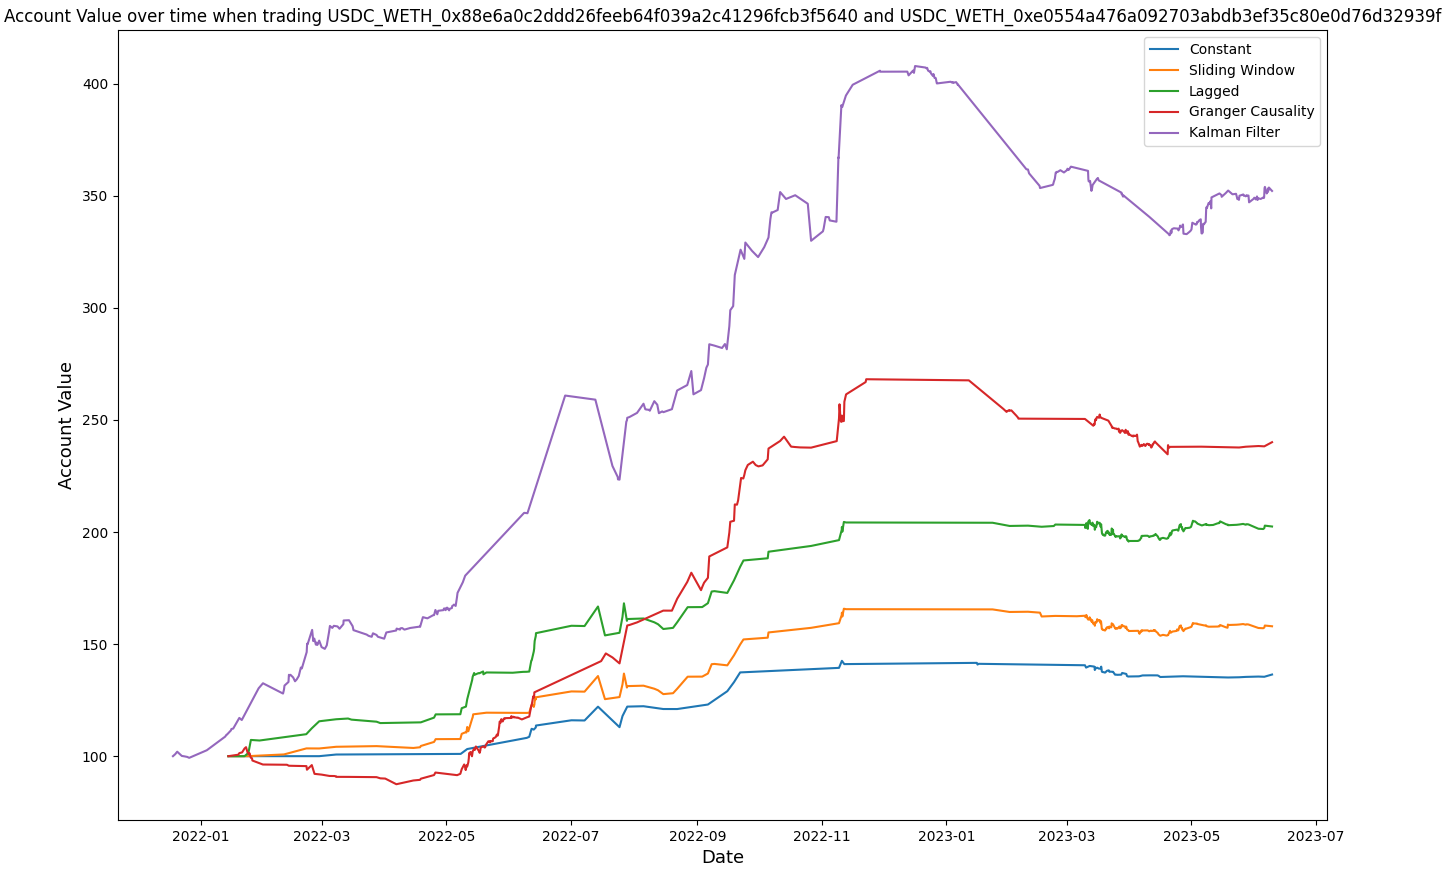
\includegraphics[width=\linewidth]{evaluation/Images/ValueHistory.png}
    \caption{Account Value over Time from backtesting Pair 0}
    \label{fig:ValueHistory}
\end{figure}

Another valuable insight can be seen in Figure \ref{fig:HedgeRatioPerStrat} where the evolution of the hedge ratio is plotted for each strategy. It can be seen that the sliding window and the granger causality strategies' hedge ratio is fairly consistent in comparison to the lagged strategy's hedge ratio. However, the Kalman Filter calculates the Hedge Ratio slightly lower and also more constant with only minor deviations, as can be seen in Figure \ref{fig:evolving_hedge_ratio_kf}. This indicates a more persistent relationship between the paired assets. The minor deviations observed in the hedge ratio can be attributed to temporary fluctuations in market dynamics or noise in the data.

\begin{figure}[H]
    \centering
    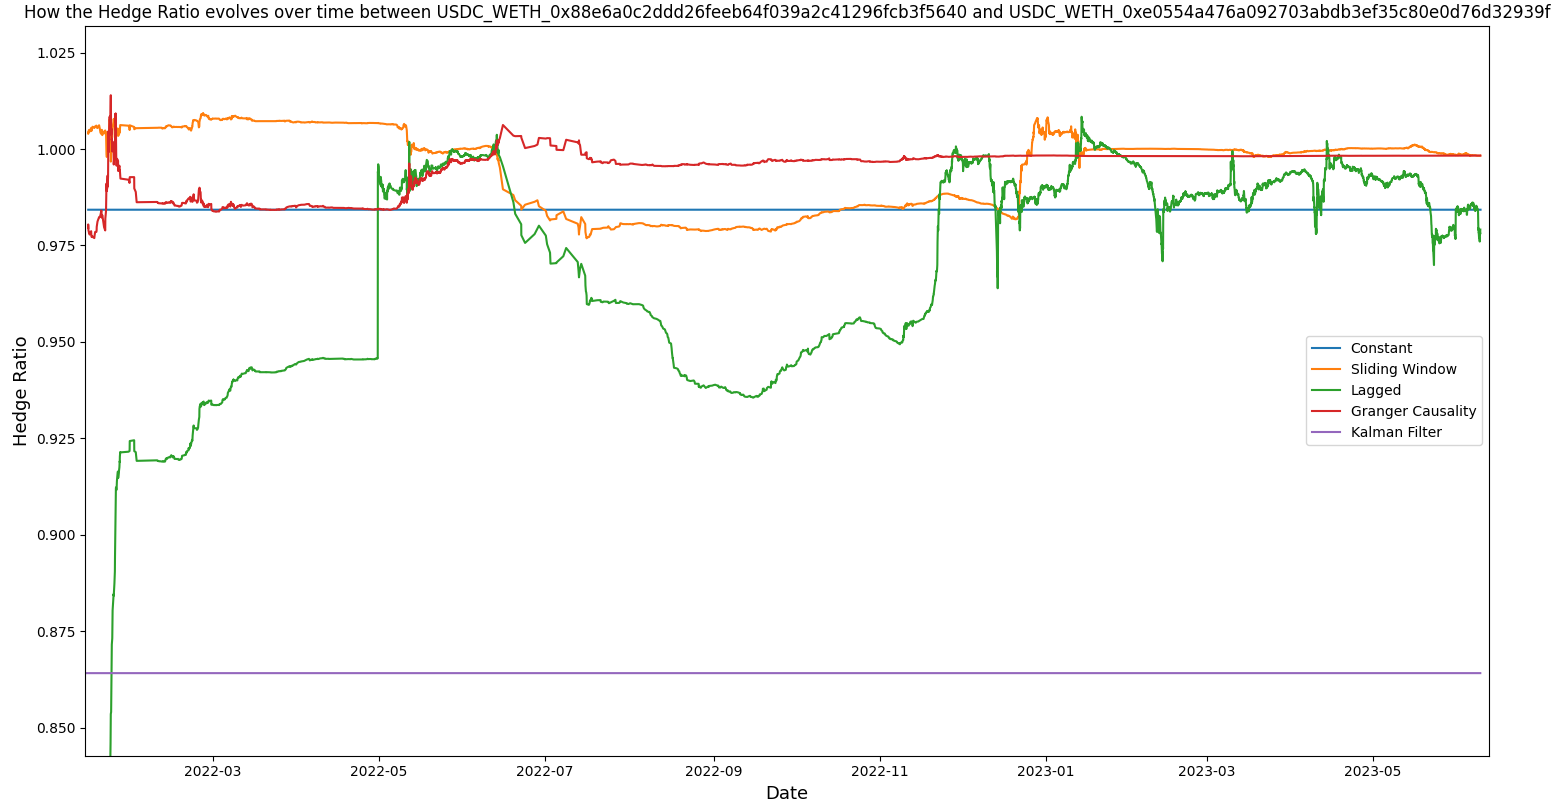
\includegraphics[width=\linewidth]{evaluation/Images/HedgeRatioPerStrat.png}
    \caption{The Hedge Ratio over time for Pair 0}
    \label{fig:HedgeRatioPerStrat}
\end{figure}


\section{Beta}
An important metric when evaluating trading strategies or investments that is used in industry is Beta, $\beta$. It measures how correlated the strategy's return is with the market return rate. It is often used as a risk-reward measure, allowing investor to make better decisions when investing, balancing the risk and reward. $\beta$ is defined as $\beta = \frac{Cov(R_M, R_S)}{Var(R_M)}$, where $R_M$ is the market's returns and $R_S$ is the strategy's or stock's returns, the higher the $\beta$ value the more correlated the strategy's return is with the market whereas a lower one, i.e. $\rightarrow - \infty$, the strategy swings the opposing direction to the market. Therefore, in risk neutral strategies, a low absolute value is ideal as it minimizes the risk.
\\[5mm]
Therefore, to analyse the $\beta$ of each strategy, the conversion from WETH to USD is used as the strategies use WETH as their base currency. As we can see in Table \ref{tab:betas}, the $\beta$s are very close to 0 indicating that the strategy's dependence on the market returns is very low. The low $\beta$ values imply that the trading strategy may be designed to generate returns based on factors other than general market movements. It suggests that the strategy relies more on specific signals, indicators, or market inefficiencies rather than the broader market conditions. This can be advantageous in certain situations, as it may allow the strategy to perform well even when the overall market is experiencing volatility or downturns.

\begin{table}[!htb]
    \centering
    \begin{adjustwidth}{-0.8in}{-0.9in}
        \begin{tabular}{|p{5em}|p{7em}|p{7em}|p{7em}|p{8em}|p{7em}|}\hline
            Pool Pair & \multicolumn{5}{|c|}{Strategies' Beta, $\beta$ - Trading from 18th December 2021 to 9th June 2023} \\\cline{1-6}
            & Constant & Sliding Window & Lagged & Granger Causality & Kalman Filter\\\cline{2-6}
            0 & -0.0011 & -0.0027987 & -0.0069576 & -0.0041534 & -0.0659306\\\cline{2-6}
            1 & -0.0006 & -0.0035851 & -0.0064798 & -0.0045647 & -0.0438947\\\cline{2-6}
            2 & -0.0002 & -0.0058748 & -0.0088261 & -0.0054649 & -0.0696322\\\cline{2-6}
            3 & -0.0006 & -0.0046291 & -0.0063303 & -0.0041478 & -0.0295122\\\cline{2-6}
            4 & -0.0007 & -0.0047436 & -0.0089812 & -0.004779 & -0.0652175\\\cline{2-6}
            5 & -0.0002 & -0.0046104 & -0.0071561 & -0.0041453 & -0.045186\\\cline{2-6}
            6 & -0.0009 & 0.0013075 & 0.0037716 & 0.0024716 & 0.0004015\\\hline\hline
            Average & -0.000626 & -0.003562 & -0.005851 & -0.003541 & -0.045567\\\hline
        \end{tabular}
    \end{adjustwidth}
    \caption{$\beta$s of each strategy \label{tab:betas}}.
\end{table}

\section{Sharpe Ratio}
Another metric that is commonly used in finance is the Sharpe Ratio, the reason for this is that it is important to evaluate how risky the strategies are compared to the risk free rate. The metric is given by the formula below:$$\text{Sharpe Ratio} = \frac{R_p - R_f}{\sigma_p}$$ Where $R_p$ is the return of a portfolio, $R_f$ is the risk-free rate and $\sigma_p$ is the standard deviation of the portfolio. A higher Sharpe ratio indicates a better risk-adjusted return, as it signifies a higher return relative to the amount of risk taken. It implies that the investment has achieved a greater excess return compared to the risk-free rate, considering the level of volatility. Conversely, a lower Sharpe ratio suggests a lower risk-adjusted return, indicating a relatively higher level of risk for the given return. The Sharpe ratio also helps investors compare different investments or strategies based on their risk adversity performance. It provides a way to assess whether the return generated by an investment adequately compensates for the level of risk taken. 
\\[5mm]
To calculate each of the strategies Sharpe Ratios, the Bank of England's interest rate of 4.5\%~\cite{boe_interest}. Table \ref{tab:sharpes} displays the sharpe ratios of each strategy, we see that the Lagged Strategy exhibits the highest hedge ratio, followed by the Granger Causality and Sliding Window strategies, while the Kalman Filter and Constant strategies have the lowest Sharpe ratios. This discrepancy can be attributed to the Kalman Filter strategy having a higher variance, indicating a greater level of risk compared to the Sliding Window, Lagged, and Granger Causality strategies. However, it is worth noting that Pool Pair 6 significantly diminishes the average Sharpe ratio due to generating losses in all strategies.We see that the average Sharpe ratio for the lagged strategy, excluding pair 6, it have a Sharpe ratio $>2$ which is considered to be `very good' and a Sharpe ratio $>1$ is considerer to be `good' according to Forbes~\cite{forbes_sharpe_ratio}. Overall, with the exception of the Constant strategy, all strategies yield desirable Sharpe ratios, indicating favourable risk-adjusted returns.

\begin{table}[!htb]
    \centering
    \begin{adjustwidth}{-0.8in}{-0.9in}
        \begin{tabular}{|p{5em}|p{7em}|p{7em}|p{7em}|p{8em}|p{7em}|}\hline
            Pool Pair & \multicolumn{5}{|c|}{Strategies' Sharpe Ratios} \\\cline{1-6}
            & Constant & Sliding Window & Lagged & Granger Causality & Kalman Filter\\\cline{2-6}
            0 & 2.1902 & 2.6611189 & 2.9222798 & 2.8685778 & 1.8181869\\\cline{2-6}
            1 & -1.2426 & 1.625967 & 2.3434127 & 1.9508066 & 1.8170602\\\cline{2-6}
            2 & -3.8312 & 2.2247116 & 2.5841394 & 2.1145482 & 1.936907\\\cline{2-6}
            3 & -1.4968 & 1.5303011 & 2.2002525 & 1.443948 & 1.6968243\\\cline{2-6}
            4 & -0.1346 & 2.1651834 & 2.5181573 & 2.264082 & 1.9388748\\\cline{2-6}
            5 & -1.4287 & 1.4943642 & 2.148777 & 1.6072208 & 1.769034\\\cline{2-6}
            6 & -1.8643 & -2.5635465 & -2.2529314 & -2.6360359 & -2.0231933\\\hline\hline
            Average & -1.115422 & 1.305443 & 1.780584 & 1.373307 & 1.279099 \\\hline
        \end{tabular}
    \end{adjustwidth}
    \caption{Sharpe Ratios of each strategy \label{tab:sharpes}}.
\end{table}

\section{Comparison with Previous results}
Overall, the strategies seem to be a desirable investment for those with enough capital however how does these invests stand against other techniques used. There has not been any research into statistical arbitrage on decentralized exchanges, with the few that have looked into trading in DEXes evaluating pure arbitrage, searching for miss-pricing and executing them. One of which found there to be little to no profitable arbitrage opportunities on various decentralised exchanges, including Uniswap, regardless of volume size~\cite{boonpeam2021arbitrage}. This happens as the pair prices as automatically adjusted based on the supply and demand, making the opportunities limited, short lived and costly. In comparing, the results from the strategies implemented in this paper do generate a profit in comparison to the cyclic arbitrage approach.
\\[5mm]
Other research into statistical approaches to arbitrage have been done on more mainstream assets such as ETFs however, they have not been experimented on cryptocurrencies. One paper used the Kalman Filter on ETFs and ETNs and found there to be an average of 25.17\% returns in 1 year in insample backtesting, however failed to generate any profit in its out of sample results~\cite{dempsey_market_2017}. The implemented Kalman Filter and Lagged trading strategies yeild a greater APR compared to this. In addition to this, another peice of research used a combination of machine learning and the Kalman Filter on assets on the BM\&FBovespa Exchange, yeilding a return of 26.13\% in the out of sample results~\cite{6974093}. In comparison, the Kalman Filter and the Lagged strategies implemented in this paper have a greater return, however the strategy implemented by Oliveira and Nóbrega, posses greater Sharpe ratio meaning the risk-adjusted returns are more favourable. To summarize, the two of the five strategies implemented out perform the current research out there on both purer forms of arbitrage, i.e. cyclic arbitrage, and also the use of Kalman Filter on other types of assets, i.e. ETFs and ETNs.
